%% This is an example first chapter.  You should put chapter/appendix that you
%% write into a separate file, and add a line \include{yourfilename} to
%% main.tex, where `yourfilename.tex' is the name of the chapter/appendix file.
%% You can process specific files by typing their names in at the 
%% \files=
%% prompt when you run the file main.tex through LaTeX.
\chapter{Surface Plasmon Resonance Sensing}

Surface Plasmon Resonance (SPR) Sensing is an optical technique used to determine a desired physical quantity using variations in the refractive index or variations in the absorption/reflection spectra. The SPR phenomena is in essence a charge density ($\rho$) wave that may occur at the interface of two media that have permittivities of opposite sign (e.g. a metal-dielectric interface), when the interface is stimulated by incident light (obeying certain resonance conditions such as wave-vector matching).  The coupled state is known as a Surface Plasmon Polariton (SPP). The charge-oscillation has an associated wave vector that achieves its maximum value at the interface and decays evanescently into the two media. 

Based on which specific parameter is used to measure the variation in the SPR wave-vector, the SPR sensors can be classified into one of five categories: angle, wavelength, intensity, phase, or polarization modulation based SPR sensors.  

\section{Surface Plasmon Polaritons and SPR}

A plasmon is a quantized unit of plasma vibration, similar to a phonon for mechanical vibrations. An example of plasma vibrations would be Surface Plasmon Polaritons (SPPs) which are generated by coupling light to electrons in an air-metal interface causing the free electrons in the metal to oscillate as a whole. This type of coupling of light to electrons allows for the breaking of the diffraction limit for the localization of light, thus allowing for light at higher wavelengths to resolve sub-wavelength features. 

Resonant excitation of SPPs (known as SPRs), are sensitive to variations in the refractive index of materials and as such are very useful in sensing applications. In particular, SPR sensing can be used to detect small fluctuations in the refractive index near the interface (where the SPR wave is the strongest); this particular configuration of the SPR sensor is known as an `affinity' SPR sensor. Such a sensor is of great use when dealing with bio-molecules since ``concentrations of analytes of interest in biological samples are in the femtomolar-to-nanomolar range'' but ``time required for analysis can be impractically long'' \cite{plasmon_future_bio}. However, as stated in \cite{plasmon_future_bio}, the process can be significantly expedited by using a flow-through geometry where the analyte solution is passed over the sensing surface - reducing the time taken for analysis.  

\subsection{Surface Plasmon Resonance}

From hereon we will only be considering metal-dielectric interfaces. Other configurations are possible but remain outside the scope of this thesis. \\
\\
The SPR phenomena is basically a free-electron wave excited by p-polarized incident light. This charge density oscillation is associated with an electromagnetic wave (known as the Surface Plasma Wave or SPW) which is also p-polarized. If we were to assume an interface between a semi-infinite dielectric and a semi-infinite metal, then the propagation constant of the SPW ($\beta$) is given by:

\begin{equation}\label{basic_SPR}
\beta = k \sqrt{\frac{\epsilon_m n_s^2}{\epsilon_m + n_s^2}}
\end{equation}

Where $k$ is the free space wave number, $\epsilon_m = \epsilon_{mr} + j \epsilon_{mi}$ is the relative permittivity of the metal, and $n_s$ is refractive index of the dielectric \cite{SPR_sensor_review}.

It is apparent from \autoref{basic_SPR} that an SPR wave way be supported by a configuration as long as the denominator ($\epsilon_m + n_s^2$) remains positive \footnote{Technically, the real part of the denominator should remain positive.}. This condition is met by many combinations of metals and dielectrics, but the most common metals used are gold and silver. Note that the generated SPW is heavily concentrated in the dielectric region and less so in the metal region. This is mainly due to the high degree of attenuation experienced by the SPW in the metal. \footnote{There are some first order approximations of electrons in metals (based on the free electron model of an electron gas) that can be used to approximate $\epsilon_m$. It is however important to note that such models neglect attenuation.}

From \autoref{basic_SPR} we may also get the skin depth ($\delta_{skin}$) of the SPW - that is the distance over which the amplitude drops to $\frac{1}{e}$ of its original value - given by:

\begin{equation}\label{skin_depth}
\delta_{skin} = \frac{1}{\Im \lbrace\beta \rbrace }
\end{equation}

\subsection{SPR Prism Geometries}

Due to the high degree of attenuation of the SPW in both the dielectric and metallic media - leading to a very limited penetration depth of the evanescent SPW - the sensing operation has to be carried out extremely close to the metal-dielectric interface. Thus it is essential that the system used to generate the SPW also be the system used to examine the SPR fluctuations. This has led to the development of extremely specialized SPR geometries.  

\subsubsection{Evanescent Waves}

If a circular beam of light is incident onto a totally internally reflecting surface, it illuminates an ellipse on that surface. Only within the ellipse is an evanescent wave induced, i.e. an evanescent wave is induced only on the illuminated area of the totally internally reflecting surface. At the boundary of the illuminated surface exists a transitional area where the evanescent wave decays to zilch. The width of this transitional area is on the order of the incident light's wavelength. 

For p-polarized incident light, the electric fields of the incident, reflected, and transmitted waves at an interface are not collinear. Careful application of Snell's law and the Fresnel equations immediately output the transmission \& reflection characteristics for the sub-critical regime. 

\begin{figure}
\centering
	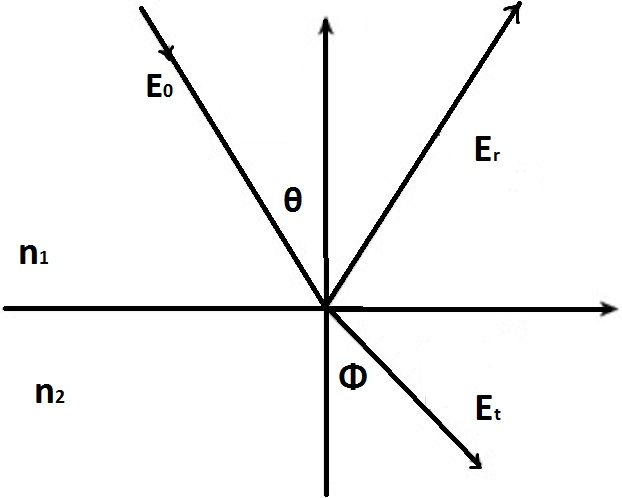
\includegraphics[width=0.75\textwidth]{TIR.png}
\caption{Figure showing sub-critical total internal reflection}
\label{fig:TIR}
\end{figure}

At the critical angle of the interface we find that this set of relations hold:

\begin{eqnarray}\label{super_crit_TIR}
E_x = 0 \\
E_y = 2E_0 \\
E_z = 2 \frac{n_1}{n_2} E_0
\end{eqnarray}

Where $n_1$, $n_2$, $E_0$ are the refractive indexes of the media surrounding the interface and incident electric field intensity respectively (as visible in \autoref{fig:TIR}). 

That $E_z$ only depends on the refractive indexes of the media implies that choosing the media correctly would allow for the $z$-component of the evanescent wave to be stronger than the electric field of the incident wave \cite{ATR_book}. Indeed, a simple calculation shows that in going from Silicon Dioxide ($n$ = 1.4585) to gold ($n$ = 0.27049) \cite{ref_index_db}, there is approximately a 5-fold increase in the evanescent wave's strength compared to the incident wave. 

Within the super-critical regime \footnote{ In this paragraph only with cases where the materials have real permittivities ($n_1$, $n_2 \in \Re$) are dealt with.} it is sufficient to note that internal reflection is approximately total. It is exactly total for a non-absorbing rarer medium ($n_2<n_1$ and  $n_1, n_2 \in \Re$).

Furthermore, the evanescent wave thus formed travels along the interface extending slightly into the rarer media (in actuality it will also extend into the denser media but can be neglected to an first order approximation).

\subsubsection{Attenuated Total Reflection (ATR)}

In reality, some of the evanescent wave is absorbed (due to complex refractive indexes) and thus the reflection is not really total. Simply put, the reflectance of the interface has troughs corresponding to those wavelengths that are absorbed by the rarer medium. At these specific wavelengths the total reflectance is said to be attenuated - hence the name Attenuated Total Reflection \cite{ATR_book}. 

ATR Spectroscopy is similar to transmission spectroscopy and relies on the absorption of part of the evanescent wave by an absorbing material. That is, when an absorbing material is brought in contact with a totally reflecting interface, it absorbs some of the intensity of the evanescent wave and thus attenuates the reflected intensity. Profiling this reflected intensity allows one to generate an `absorption' spectra and hence understand how optical parameters vary in the absorbing material.

Assuming that $n_1 \in \Re$ and $n_2 \in \mathbb{C}$ \footnote{As with a metal-dielectric interface.} we may derive the expression for the super-critical internal reflectance of p-polarized light:

\begin{equation}
R_p = \left| \frac{n_2^2 \cos \theta - j n_1 \sqrt{n_1^2 \sin ^2 \theta - n_2^2}}{n_2^2 \cos \theta + j n_1 \sqrt{n_1^2 \sin ^2 \theta - n_2^2}}\right|^2
\end{equation}\label{super_crit_ref}

This equation is somewhat intractable and does not allow for in-depth understanding of the underlying physics. To gain a detailed understanding of absorption during super-critical internal reflection, there are less abstruse models such as the `Weak Absorption Model' or the `Leaky Interface Model' which barter accuracy for comprehensibility. An in-depth exploration of these models is provided in \cite{ATR_book}. 

\subsubsection{ATR Prism Geometries}

If we were to look again to \autoref{basic_SPR} and use the approximation that $\epsilon_m \approx \epsilon_{mr}$ \footnote{This is equivalent to saying $\Re\{\epsilon_m\} \approx \epsilon_m$, which is a good approximation for metals since the imaginary component of $\epsilon_m$ is usually very small.} then we see that \autoref{comp_air_SP} holds (equality is achieved as $k \rightarrow 0$).

\begin{equation}\label{comp_air_SP}
\beta_{SP} = k \sqrt{\frac{\epsilon_{mr} n_s^2}{\epsilon_{mr}+ n_s^2}} \geq \beta_{air} = k n_s
\end{equation}

It is evident that in order to excite plasmons in a resonant fashion, the momentum of the incident light has to be enhanced to match the momentum of the SPW. This momentum enhancement can be engineered using ATR in prism couplers. 

In the case of p-polarized light, the interaction may be simplified to incident light being passed through a prism made of glass to increase its momentum (and wave-number), so as to achieve resonance at a given wavelength \& angle of incident. There are two main prism coupler variants - the `Otto' configuration and the `Kretschmann' configuration. Both are shown in \autoref{fig:ATR}

\begin{figure}
\centering
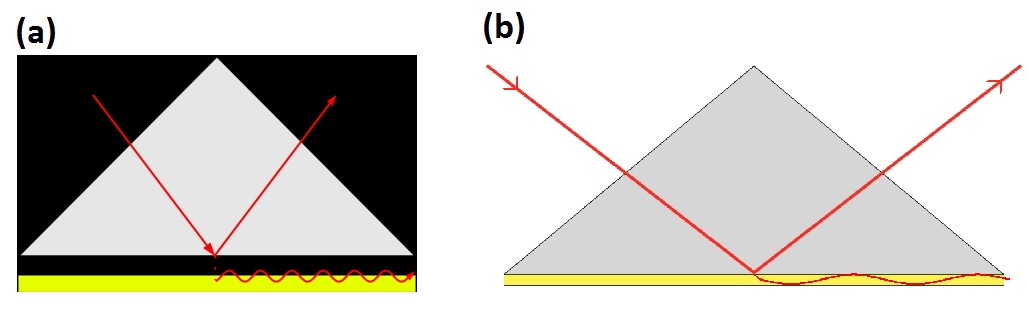
\includegraphics[width=0.75\textwidth]{ATR.jpg}
\caption{Figure showing (a) the Otto prism configuration and (b) the Kretschmann prism configuration}
\label{fig:ATR}
\end{figure}

The only significant difference between the Kretschmann setup and the Otto setup is the positioning of the metal film. In the Kretschmann setup the metal film is adhered onto the glass prism whereas, in the Otto setup, it is simply placed sufficiently close (a few 100 nm) so as to interact with the generated evanescent wave. 

The equations governing the coupling of incident light to generate a SPP are simply a consequence of wave-vector matching:

\begin{eqnarray} \label{mom_match}
\beta_{incident} = k n_{prism} \sin \theta_{SP} \\
\beta_{SP} = k \sqrt{\frac{\epsilon_m n_s^2}{\epsilon_m + n_s^2}}
\end{eqnarray}

Setting the above equations equal to each other results in \footnote{A variant of this result, including the effects of grating coupling, is available in \cite{farshid_ol}.}:

\begin{equation}\label{final_mom_eq}
\Re\left\lbrace\sqrt{\frac{\epsilon_m n_s^2}{\epsilon_m + n_s^2}}\right\rbrace = n_{prism} \sin \theta_{SP}
\end{equation}

For completeness, the equation governing grating coupling (oriented with the grating surface in the x-direction) is also provided below\footnote{The addition of grating coupling to prism coupling is a simple linear extension which will not be explained in detail in this thesis, but both are explained in great detail in \cite{complete_sp_coupling} or \cite{sp_coupling_2} if required.}:

\begin{equation}\label{grating_coupling}
\beta_x +mG = \beta^{'}_{xm}
\end{equation}

Where $m \in \mathbb{Z}$, $\beta_x$ is the component of the incident wave-vector along the grating surface, and $G = \frac{2\pi}{\lambda_g}$ is the grating wave-vector ($\lambda_g$ is the grating wave-length).

\section{SPR Sensing}

The principle behind SPR sensing is to use ATR to discern variations in the refractive index of the dielectric medium. The resonant excitation of the SPPs by incident light results in an SPW extending into the dielectric. Due to the large density of the SPW's field inside the dielectric under resonance conditions, the propagation constant (given by \autoref{basic_SPR}) is extremely sensitive to variations in the optical properties of the dielectric adjacent to the metal layer supporting the SPW (we call this dielectric layer the transducing medium). Consequently, small fluctuations in the transducing medium can be detected via SPR sensing. The requirement that the transducing medium be adjacent to the metal layer is a result of the limited penetration depth of the SPW into the dielectric.

To put this more mathematically:

\begin{equation}
\delta \beta_{SP} = \frac{\partial \beta_{SP}}{\partial n_s} \delta n_s = \frac{k n_s (\epsilon_{mr} +j \epsilon_{mi} )^2}{\sqrt{\frac{n_s^2 (\epsilon_{mr} +j \epsilon_{mi} )}{j
   \epsilon_{mi} +n_s^2+\epsilon_{mr} }} \left(j \epsilon_{mi} +n_s^2+\epsilon_{mr} \right)^2} \delta n_s
\end{equation}

Under the assumption that $\epsilon_{mi}$ is negligible this gives:

\begin{equation}
\delta \beta_{SP} = \frac{k \epsilon_{mr}  \sqrt{\frac{n_s^2 \epsilon_{mr}}{n_s^2+\epsilon_{mr} }}}{n_s^3+n_s \epsilon_{mr}} \delta n_s
\end{equation}

Using a Laurent expansion (about $\epsilon_{mr} = \infty$) this can be simplified further to:

\begin{equation}\label{SPR_var}
\delta \beta_{SP} = \frac{\partial \beta_{SP}}{\partial n_s} \delta n_s \approx k \delta n_s
\end{equation}

So far we have only mentioned affinity sensors. To clarify, there are two main uses for SPR sensors: to discern variations within the `entire' dielectric region - better known as bulk sensing; or to discern variations near the interface - better known as affinity sensing.  

Based on which specific parameter is used to measure the variation in the SPR wave-vector \footnote{The terms `wave-vector' and `propagation constant' are used interchangeably.}, the SPR sensors can be classified into one of five categories: angle, wavelength, intensity, phase, or polarization modulation based SPR sensors.  

The five categories can be divided into roughly two sub-classes:

\begin{itemize}
\item Angle and wavelength modulation based sensors are primarily used to determine the resonance angle/wavelength at which a configuration has maximum coupling, ceterus paribus.
 
\item Intensity, Phase and Polarization modulation based SPR sensing is used to profile the change in the intensity, the shift in the phase, or the variation in the polarization of the incident light which couples to the SPW, ceterus paribus. 
\end{itemize}

\subsection{SPR Bio-Sensing}

Within the field of bio-sensing, SPR sensing has established itself as an extraordinarily powerful and and quantitative probe of interactions which provides a means of identifying various interactions of bio-polymers. Further, SPR sensing also allows one to assign numerical values to various associated parameters such as: interaction equilibrium constants, interaction kinetic constants, and the intrinsic energetics of the various interactions.

A modified flow-based configuration based on the Kretschmann configuration is shown in \autoref{fig:SPR_flow}. In the figure, a glass slide with a gold layer is adhered to a prism. Light passes through, couples to the gold-glass interface, reflects off the interface and passes back through the prism to a detector. Profiling the reflection against incident angle or wavelength gives a signal (real-time) proportional to the density of bio-polymer near the interface (in the adlayer). 

\begin{figure}
\centering
	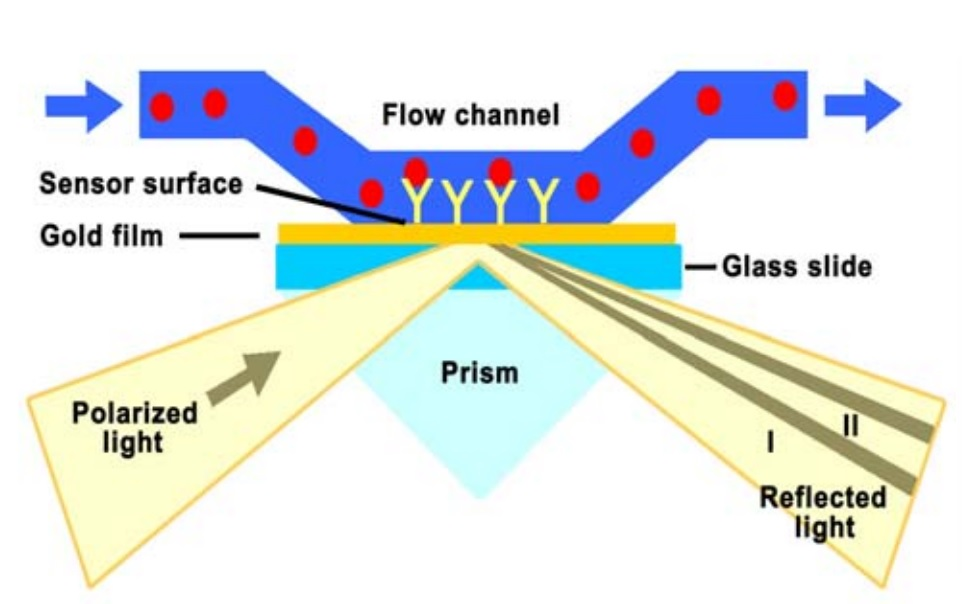
\includegraphics[width=0.75\textwidth]{SPR_flow.jpg}
\caption{A typical flow based configuration for SPR bio-sensing (taken from \cite{flow_pdf})}
\label{fig:SPR_flow}
\end{figure}

The corresponding optical response vs. time graph (sensogram) is shown in \autoref{fig:SPR_kin}. It is important to start with a stable baseline (generated by running pure buffer solution) against which one can compare variations in the optical response. The gold sensing surface is coated with targeted bio-receptors (mostly specific to single analyte molecule). Analyte molecules are injected and then left alone to achieve interaction equilibrium (the association stage - generating an adlayer). During this stage there may be a few molecules that non-specifically attach to the bio-receptors. To get rid of the non-targeted molecules that affixed themselves to the bio-receptors, the buffer solution is run through the system (we are now at the dissociation stage). At this point we should have pure dissociation as per Le Chatelier's principle (``If a dynamic equilibrium is disturbed by changing the conditions, the position of equilibrium moves to partially reverse the change.''). We then have a regeneration stage to get the system back to its stable baseline.

\begin{figure}
\centering
	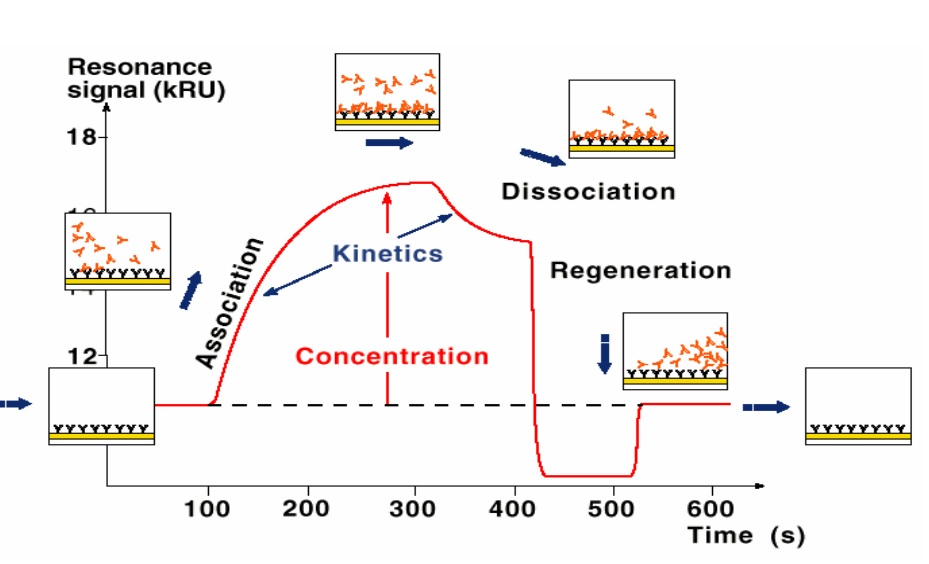
\includegraphics[width=0.75\textwidth]{SPR_kin.jpg}
\caption{A response-time graph of a typical SPR bio-sensing experiment (taken from \cite{flow_pdf})}
\label{fig:SPR_kin}
\end{figure}

\section{Motivation for a Dielectric Grating based SPR}

In an SPR bio-sensor we aim to acquire information regarding the adlayer in the form of the adlayer's thickness ($d_a$) and the adlayer's index of refraction ($n_a$). However, the optical response of the SPR sensor also depends on factors such as the bulk analyte solution's index ($n_b$). This is due to the evanescent nature of the SPW and its appreciable interaction with media beyond the thin adlayer. One way to decouple this information is to use an additional reference channel (to keep track of variations in $n_b$). The main drawback of this ad-hoc method is that it's hard to implement and requires that every sensing channel be replicated as perfectly as possible, significantly hindering the use of the SPR sensor in high-throughput systems. Even if ideal conditions were somehow possible $n_a$ still cannot be easily decoupled from $d_a$ with a reference channel. 

A Dielectric Grating based SPR (DGSPR) sensor is precisely what it sounds like. Developed by Bahrami et al., it's basically a Kretschmann configuration with an additional dielectric grating on top of the gold layer. This novel configuration allows for multiple stable SPR modes (you can achieve 3, 5, or even 7 mode spectroscopy). Given 3+ different continuous (or rather semi-continuous) measurements you can decouple $d_a$, $n_a$, and $n_b$ from each other (if you use 7 modes then you could decouple a lot more extraneous factors). The only caveat with the DGSPR based sensor is that the normalized system matrix, i.e. the matrix containing the coupled set of differential equations that govern the sensing system, cannot be singular. This is easy enough to verify and the method to do so, along with an in-depth discussion of the DGSPR sensor, is provided in \cite{farshid_ol}.

In this thesis, from here onward only the 3 mode configuration will be discussed (two p-polarized modes and one s-polarized mode). The other modes are theoretically possible but somewhat fiddly to actually realize and hence outside the scope of this thesis. 

\section{Summary}

In this chapter a brief introduction to SPR based sensing has been provided along with the motivation for the DGSPR sensor. The next chapter will deal with the actual DGSPR design and its brute-force optimization.